\documentclass[11pt,a4paper]{article}
\usepackage[margin=21mm,headheight=14pt]{geometry}
\usepackage[T1]{fontenc}
\usepackage{lmodern,microtype,amsmath,amssymb,graphicx,booktabs,longtable}
\usepackage[table]{xcolor}
\usepackage{enumitem,fancyhdr,caption,listings,xurl,hyperref}
\definecolor{teal}{HTML}{197A78}
\definecolor{ink}{HTML}{172A3A}
\definecolor{pale}{HTML}{EFF5F5}
\hypersetup{colorlinks=true,linkcolor=teal,urlcolor=teal,citecolor=teal,
  pdftitle={Friendship Structure in an Anonymised Facebook Network},
  pdfauthor={Mervine Muganguzi},
  pdfsubject={Network analysis of SNAP Facebook friend network 3980 using Python}}
\pagestyle{fancy}
\fancyhf{}
\fancyhead[L]{\small\textcolor{teal}{Facebook friendship network 3980}}
\fancyhead[R]{\small Statistical Analysis and Forecasting}
\fancyfoot[R]{\small\thepage}
\renewcommand{\headrulewidth}{0.4pt}
\setlength{\parindent}{0pt}
\setlength{\parskip}{5pt}
\setlist[itemize]{leftmargin=*,itemsep=2pt,topsep=3pt}
\setlist[enumerate]{leftmargin=*,itemsep=2pt,topsep=3pt}
\captionsetup{font=small,labelfont={bf,color=teal},skip=5pt}
\graphicspath{{../figures/}}
\lstset{language=Python,basicstyle=\ttfamily\fontsize{7.6}{9.1}\selectfont,
  keywordstyle=\color{teal}\bfseries,commentstyle=\color{gray},
  stringstyle=\color{ink},numbers=left,numberstyle=\tiny\color{gray},
  numbersep=7pt,breaklines=true,breakatwhitespace=true,showstringspaces=false,
  columns=fullflexible,keepspaces=true,frame=single,rulecolor=\color{black!15},
  xleftmargin=12pt,framexleftmargin=5pt,tabsize=4}
\newcommand{\Nnodes}{59}
\newcommand{\Nedges}{146}
\newcommand{\Rawrows}{292}
\newcommand{\MeanDistance}{2.567}
\newcommand{\Diameter}{5}
\newcommand{\MainQ}{0.4139}
\newcommand{\FullQ}{0.4576}
\newcommand{\Qlow}{0.4064}
\newcommand{\Qhigh}{0.4151}
\newcommand{\ARIlow}{0.441}
\newcommand{\PythonVersion}{3.12.14}
\newcommand{\NetworkXVersion}{3.7}
\newcommand{\MatplotlibVersion}{3.10.8}
\newcommand{\NumpyVersion}{2.3.5}
\newcommand{\ScipyVersion}{1.17.0}
\newcommand{\AverageClustering}{0.4069}
\newcommand{\Transitivity}{0.4500}
\newcommand{\CliquePeople}{15}
\newcommand{\FourRunCount}{11}
\newcommand{\FiveRunCount}{19}
\begin{document}
\thispagestyle{plain}
{\small\textcolor{teal}{STATISTICAL ANALYSIS AND FORECASTING\quad /\quad NETWORK ANALYSIS}}\\[8pt]
{\LARGE\bfseries\textcolor{ink}{Friendship Structure in an\\[2pt] Anonymised Facebook Network}}\\[7pt]
{\large A reproducible analysis of SNAP friend network 3980 using Python}\\[5pt]
{\normalsize\textbf{Mervine Muganguzi}}\\[4pt]
{\small 6 November 2026}

\subsection*{Abstract}
This report examines observed friendships among \Nnodes{} anonymised Facebook users.
The graph contains \Nedges{} unique, undirected relationships and satisfies the
assignment's minimum of 30 people. Five centrality measures, exact clique
enumeration and Louvain community detection describe different aspects of its
structure. Person 4030 has the highest degree and eigenvector centrality, while
person 4023 leads closeness, betweenness and PageRank. The maximum clique size is
six, with six overlapping cliques of that size covering 15 distinct people.
Community boundaries vary across
random seeds, so they are interpreted as algorithmic groupings. Prepared data,
complete code and numerical outputs accompany the report.

\section{Aim and dataset preparation}
The aim is to identify well-connected people, people who connect different parts
of the graph, fully connected friendship groups and broader communities.
The data are from Stanford's SNAP \emph{Social circles: Facebook} collection,
originally studied by McAuley and Leskovec~\cite{snap,mcauley}.

The selected network belongs to anonymised ego user 3980. Only this user's
friends and the recorded friendships \emph{among those friends} are analysed.
The ego is excluded: adding the ego would create a guaranteed connection to
every friend and change the question being studied. Anonymous numerical IDs
already replace personal identifiers, so names or invented initials are unnecessary.
The network was selected for its friendship interpretation and manageable size;
it is not a random sample of Facebook users.

\textbf{Preparation procedure.}
\begin{enumerate}
\item Read the complete roster from \texttt{3980.feat}, using only its first
column of anonymised IDs. Profile feature values are not used.
\item Read \texttt{3980.edges}. Its \Rawrows{} rows record each undirected
friendship twice. Sort each endpoint pair and remove repeated pairs to obtain
\Nedges{} unique edges. No self-loops occur.
\item Add all \Nnodes{} roster nodes before adding edges. Reading only the edge
file would retain 52 people and omit seven isolated nodes.
\item Save \texttt{nodes.csv} and \texttt{edges.csv}, retain source metadata and
the archive's SHA-256 checksum, and use sorted inputs for reproducibility.
\end{enumerate}

The graph represents an observed subnetwork. An isolate has no recorded tie to
the other selected friends; this does not mean that the person has no friends
elsewhere. Source circle memberships are not used; the groups below are detected
from friendship edges. The archive and prepared CSV files allow the analysis to run offline.
The data access date is 6 November 2026.

\clearpage
\section{Methods and mathematical definitions}
\subsection{Graph notation and basic statistics}
Following the lecture's graph terminology~\cite{lecture}, let $G=(V,E)$ be a
simple, unweighted, undirected graph, with $N=|V|$ people,
$m=|E|$ friendships and adjacency matrix $A$. Thus $A_{ij}=1$ when people $i$
and $j$ are friends, and zero otherwise. The degree is $k_i=\sum_j A_{ij}$.
Network density and average degree are
\begin{equation}
\rho=\frac{2m}{N(N-1)},\qquad \bar{k}=\frac{2m}{N}.
\end{equation}
For vertices in the same connected component, $d(i,j)$ is the shortest-path
length in number of edges. The diameter is the largest such distance. A finite
whole-network diameter or average over all pairs is not reported for this
disconnected graph. These distances are calculated for the largest connected
component $H$, which contains 44 nodes.

If $t_i$ is the number of triangles containing node $i$, its local clustering
coefficient is $C_i=2t_i/[k_i(k_i-1)]$ for $k_i\geq2$, and zero otherwise.
Average clustering is $N^{-1}\sum_i C_i$. Global transitivity is
$3T/\sum_i\binom{k_i}{2}$, where $T$ is the number of triangles.

\subsection{Centrality measures}
All primary centralities are calculated on the full 59-node graph. A second CSV
recalculates them on $H$ with its own normalisation. The formulas follow the
NetworkX definitions~\cite{nxcentrality}.

\textbf{Degree centrality} measures direct connections:
\begin{equation}
C_D(i)=\frac{k_i}{N-1}.
\end{equation}
It is a measure of local connectedness; it does not by itself establish social
influence.

\textbf{Closeness centrality} measures short-path reachability. Let $R_i$ be the
other nodes reachable from $i$ and $r_i=|R_i|$. The Wasserman--Faust correction
accounts for disconnectedness:
\begin{equation}
C_C(i)=\frac{r_i}{N-1}\frac{r_i}{\sum_{j\in R_i}d(i,j)}.
\end{equation}
An isolate receives zero. Without the first factor, a node in a tiny component
could appear highly central merely because the few reachable nodes are nearby.

\textbf{Betweenness centrality} measures shortest-path bridging. If $\sigma_{st}$
is the number of shortest paths between $s$ and $t$, and $\sigma_{st}(i)$ counts
those passing through $i$, the normalised undirected measure is
\begin{equation}
C_B(i)=\frac{2}{(N-1)(N-2)}
\sum_{\substack{s<t,\;s,t\ne i\\\sigma_{st}>0}}
\frac{\sigma_{st}(i)}{\sigma_{st}}.
\end{equation}
The sum includes reachable pairs only; unreachable pairs contribute zero.
Endpoints are excluded from path counts.

\textbf{Eigenvector centrality} gives more weight to ties to other central nodes:
\begin{equation}
Ax=\lambda_{\max}x,\qquad x_i\geq0,\qquad \sum_i x_i^2=1.
\end{equation}
For this disconnected graph, the dominant eigenvector concentrates on the
44-node component: its leading adjacency eigenvalue is approximately 9.455,
compared with 3.000 for the next-largest value among the other components.
Scores outside it are effectively zero and cannot usefully rank people in those
smaller components.

\clearpage
\subsection*{Centrality measures (continued)}
\textbf{PageRank} describes the stationary probability of a random walk with
uniform teleportation. Each friendship is treated as two reciprocal directions.
For damping factor $\alpha=0.85$,
\begin{equation}
p_i=\frac{1-\alpha}{N}+\alpha\left[
\sum_{j\in\mathcal{N}(i)}\frac{p_j}{k_j}
+\frac{1}{N}\sum_{j:k_j=0}p_j\right],\qquad \sum_i p_i=1.
\end{equation}
The final term redistributes mass from isolates uniformly. Consequently every
node has positive PageRank. This is an undirected friendship interpretation,
not evidence of one-way popularity~\cite{nxpagerank}.

\subsection{Cliques}
A set $S\subseteq V$ is a clique when all distinct pairs are connected:
\begin{equation}
A_{ij}=1\quad\text{for every distinct }i,j\in S,
\qquad \omega(G)=\max_{S\text{ is a clique}}|S|.
\end{equation}
A \emph{maximal} clique cannot be enlarged by adding a node. A \emph{maximum}
clique has the largest size in the entire graph. These terms are different:
a small clique can be maximal without being maximum.

All cliques are enumerated to count groups by size. Maximal cliques are found
with \texttt{nx.find\_cliques}, which uses a Bron--Kerbosch-based algorithm;
the largest of these give the exact clique number~\cite{nxcliques}.
Counts are feasible for this small graph. Cliques can overlap.

\subsection{Community detection and sensitivity}
A community is a group with relatively concentrated internal connections; it
does not require every pair to be friends. Louvain is a heuristic that seeks
large modularity~\cite{blondel,nxlouvain}:
\begin{equation}
Q=\frac{1}{2m}\sum_{i,j}\left(A_{ij}-\gamma\frac{k_i k_j}{2m}\right)
\mathbf{1}(c_i=c_j),\qquad \gamma=1.
\end{equation}
Here $c_i$ is the community of node $i$. The null-model term represents expected
ties under a degree-preserving model. Louvain alternates node moves that improve
$Q$ with aggregation of communities into a smaller graph. It does not guarantee
the globally optimal partition or a unique social grouping.

The primary run uses seed 42. Separate partitions are fitted on the full graph
and on $H$. They optimise different graphs, so their labels and modularity values
are not directly interchangeable. On $H$, seeds 0--29 assess sensitivity to node
processing order. The adjusted Rand index (ARI) compares each partition with
seed 42 after correcting pairwise agreement for chance. If $n_{uv}$ counts
shared members of groups $u$ and $v$ in the two partitions, let
$I=\sum_{u,v}\binom{n_{uv}}2$, $R=\sum_u\binom{a_u}2$ and
$S=\sum_v\binom{b_v}2$, where $a_u$ and $b_v$ are their group sizes and
$n_H=|V(H)|=44$. Then
\begin{equation}
\mathrm{ARI}=\frac{I-E}{(R+S)/2-E},\qquad E=\frac{RS}{\binom{n_H}{2}}.
\end{equation}
An ARI of 1 means identical assignments; values near 0 indicate chance-level
agreement under fixed group sizes. Layouts also use seed 42. Display positions
are not geography or numerical shortest-path distances.

\clearpage
\section{Results: overall structure}
\begin{table}[h!]
\centering\small
\begin{tabular}{llr}
\toprule
Scope & Statistic & Value \\
\midrule
Whole graph & People & 59 \\
 & Unique friendships & 146 \\
 & Density & 0.0853 \\
 & Average degree & 4.949 \\
 & Connected components & 11 \\
 & Isolates & 7 \\
Main component & People & 44 \\
 & Friendships & 138 \\
 & Mean shortest-path distance & 2.567 \\
 & Diameter & 5 \\
\bottomrule
\end{tabular}

\caption{Basic properties, with whole-network and main-component scopes
separated. Distance statistics apply only to the 44-node component.}
\end{table}
The largest component contains 44 of 59 people (74.6\%) and 138 of 146 edges
(94.5\%). The other connected groups contain four, two and two people; seven
additional components are single isolated nodes. Overall, 8.53\% of possible
friendship pairs are observed. Mean local clustering is \AverageClustering{}
and transitivity is \Transitivity{}, both calculated on all 59 nodes. These
describe concentration of ties around groups; they do not establish statistical
significance against a random-network model.
\begin{figure}[h!]
\centering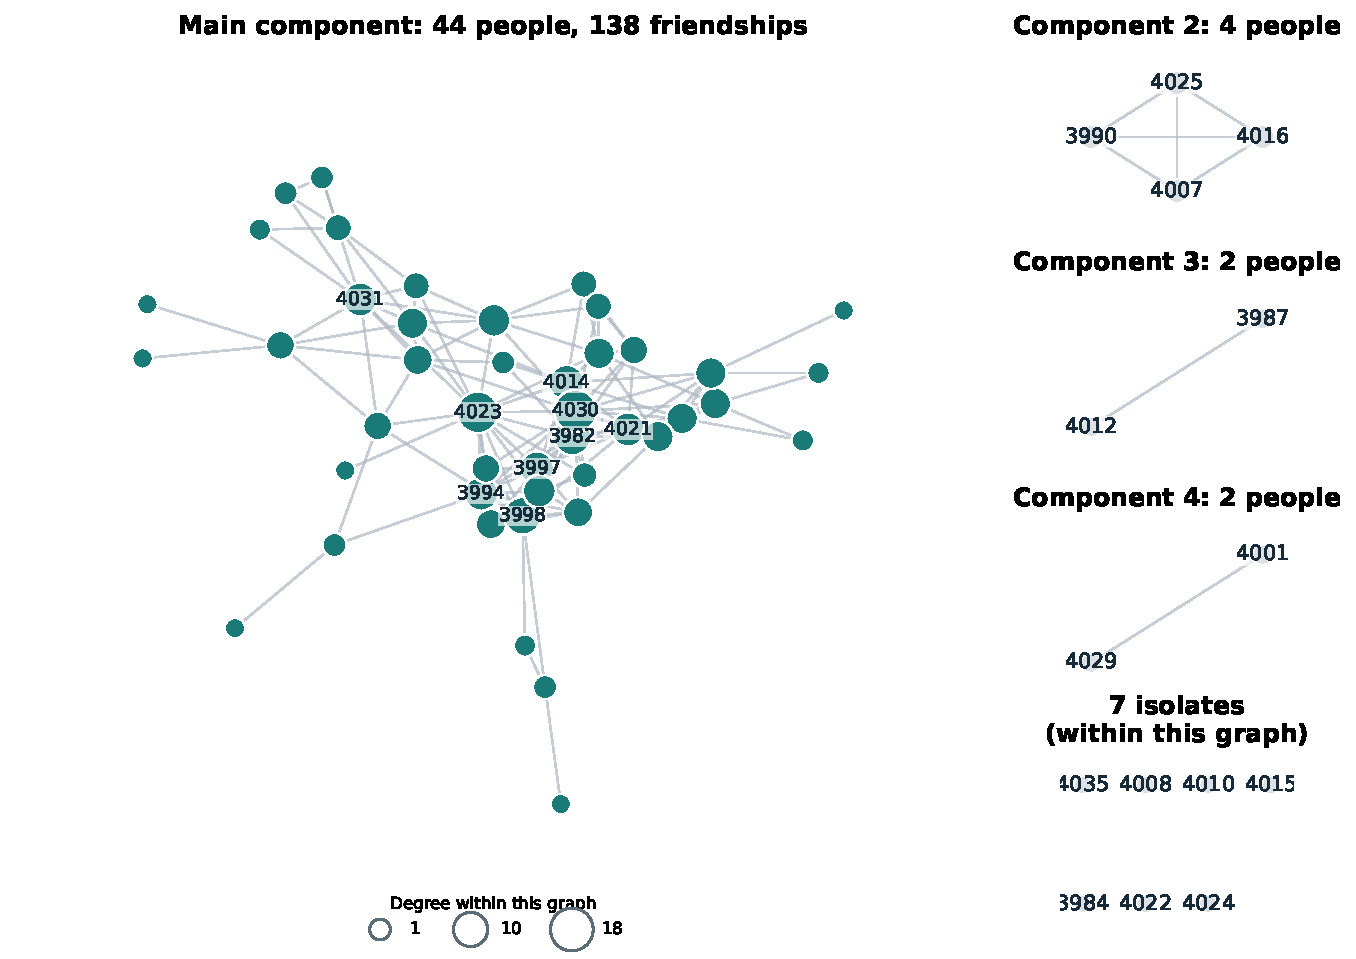
\includegraphics[width=\linewidth]{01_network_overview.pdf}
\caption{All 59 people, with disconnected components displayed separately.
Labels are anonymised source IDs. To avoid crowding, the main panel labels people
with degree at least ten or in the top five for betweenness. The size key gives
degree within this graph; positions and panel separation are illustrative.
Smaller components show every ID.}
\label{fig:overview}
\end{figure}
Within the main component, the mean shortest path is \MeanDistance{} edges and
the diameter is \Diameter{}. These figures describe reachability inside this
observed component, not separation across Facebook as a whole.

\clearpage
\section{Results: centrality}
\begin{table}[h!]
\centering\small
\begin{tabular}{rrrrrrr}
\toprule
ID & $k$ & $D$ & $C$ & $B$ & $E$ & $P$ \\
\midrule
4030 & 18 & 0.3103 & 0.4035 & 0.1042 & 0.3544 & 0.0447 \\
4023 & 17 & 0.2931 & 0.4195 & 0.1228 & 0.3211 & 0.0453 \\
3982 & 13 & 0.2241 & 0.3707 & 0.0283 & 0.2949 & 0.0328 \\
3998 & 13 & 0.2241 & 0.3795 & 0.0886 & 0.2634 & 0.0363 \\
4014 & 11 & 0.1897 & 0.3795 & 0.0522 & 0.2277 & 0.0290 \\
3994 & 10 & 0.1724 & 0.3542 & 0.0316 & 0.2427 & 0.0267 \\
3997 & 10 & 0.1724 & 0.3503 & 0.0047 & 0.2609 & 0.0252 \\
4021 & 10 & 0.1724 & 0.3356 & 0.0178 & 0.2262 & 0.0258 \\
4031 & 10 & 0.1724 & 0.3391 & 0.0776 & 0.0967 & 0.0324 \\
4004 & 9 & 0.1552 & 0.3582 & 0.0292 & 0.1427 & 0.0252 \\
\bottomrule
\end{tabular}

\caption{Ten highest-degree people, ordered by degree then ID. $k$ is raw
degree; $D$, $C$, $B$, $E$ and $P$ denote normalised degree, corrected closeness,
normalised betweenness, unit-length eigenvector centrality and PageRank.
All scores use the full 59-node graph.}
\end{table}
\begin{figure}[h!]
\centering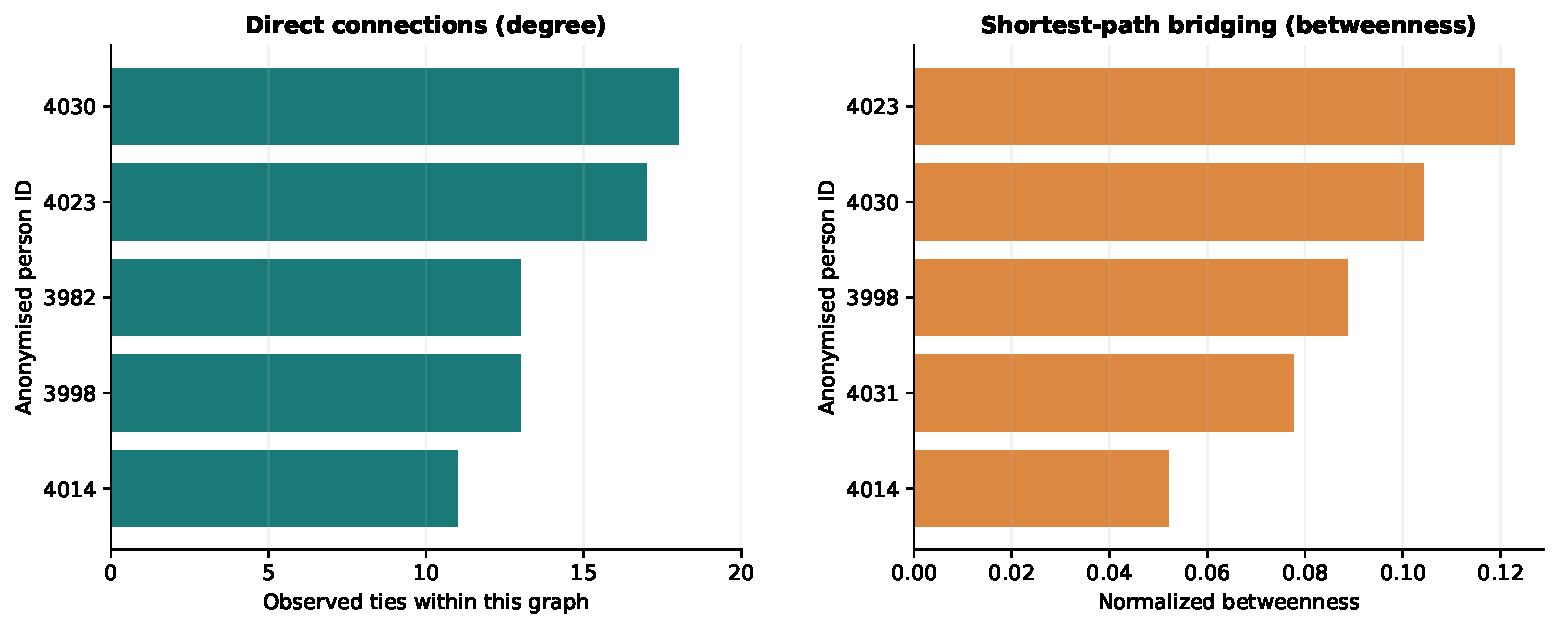
\includegraphics[width=\linewidth]{03_centrality_comparison.pdf}
\caption{The top five people differ when centrality measures direct ties or
shortest-path bridging. Degree ties in the top-five display are broken by ID.}
\end{figure}
\textbf{Direct ties and bridging are different.} Person 4030 has 18 neighbours
within this selected graph and the highest degree centrality ($18/58=0.3103$), together with the
highest eigenvector centrality. Person 4023 has 17 friends but the highest
betweenness (0.1228), corrected closeness (0.4195) and PageRank (0.0453).
Its betweenness rank describes its fractional contribution to shortest paths
between other people in this graph.

\textbf{Equal degree can hide different roles.} People 3982 and 3998 both have
13 friends, but their betweenness scores are 0.0283 and 0.0886 respectively.
Person 3998 therefore ranks higher as a shortest-path intermediary, with the
same number of direct ties. These are structural roles;
the data do not observe actual communication, influence or information flow.

The seven isolates have zero degree, closeness and betweenness. Their PageRank
is positive because of teleportation. Full results for all people appear in
Appendix~\ref{app:centrality}; a separate CSV recalculates all five measures on $H$.

\clearpage
\section{Results: cliques}
\begin{minipage}[t]{0.43\linewidth}
\vspace{0pt}
\small\begin{tabular}{rrr}
\toprule
Size & All & Maximal \\
\midrule
3 & 168 & 19 \\
4 & 108 & 12 \\
5 & 39 & 7 \\
6 & 6 & 6 \\
\bottomrule
\end{tabular}

\captionof{table}{Clique counts in the whole 59-node graph, for groups of at
least three people. Counts include overlapping groups.}
\end{minipage}\hfill
\begin{minipage}[t]{0.53\linewidth}
\vspace{0pt}
The graph contains 168 triangles, 108 four-person cliques and 39 five-person
cliques. There are six maximum cliques, each with six people, so $\omega(G)=6$.
Each has all $\binom{6}{2}=15$ possible friendships.

There are 44 maximal cliques of size at least three. The six maximum cliques
overlap and together cover \CliquePeople{} distinct people. For example, the
first two maximum cliques below share five people.
\end{minipage}
\begin{table}[h!]
\centering\small\begin{tabular}{rl}
\toprule
Clique & Anonymised person IDs \\
\midrule
1 & 3981, 3994, 3997, 3998, 4009, 4019 \\
2 & 3981, 3994, 3997, 3998, 4009, 4023 \\
3 & 3981, 3994, 3997, 3998, 4018, 4023 \\
4 & 3982, 3994, 3997, 3998, 4009, 4023 \\
5 & 3982, 3994, 3997, 4009, 4023, 4030 \\
6 & 3986, 4000, 4017, 4021, 4026, 4030 \\
\bottomrule
\end{tabular}

\caption{All six maximum cliques, in reproducible lexicographic order.}
\end{table}
\begin{figure}[h!]
\centering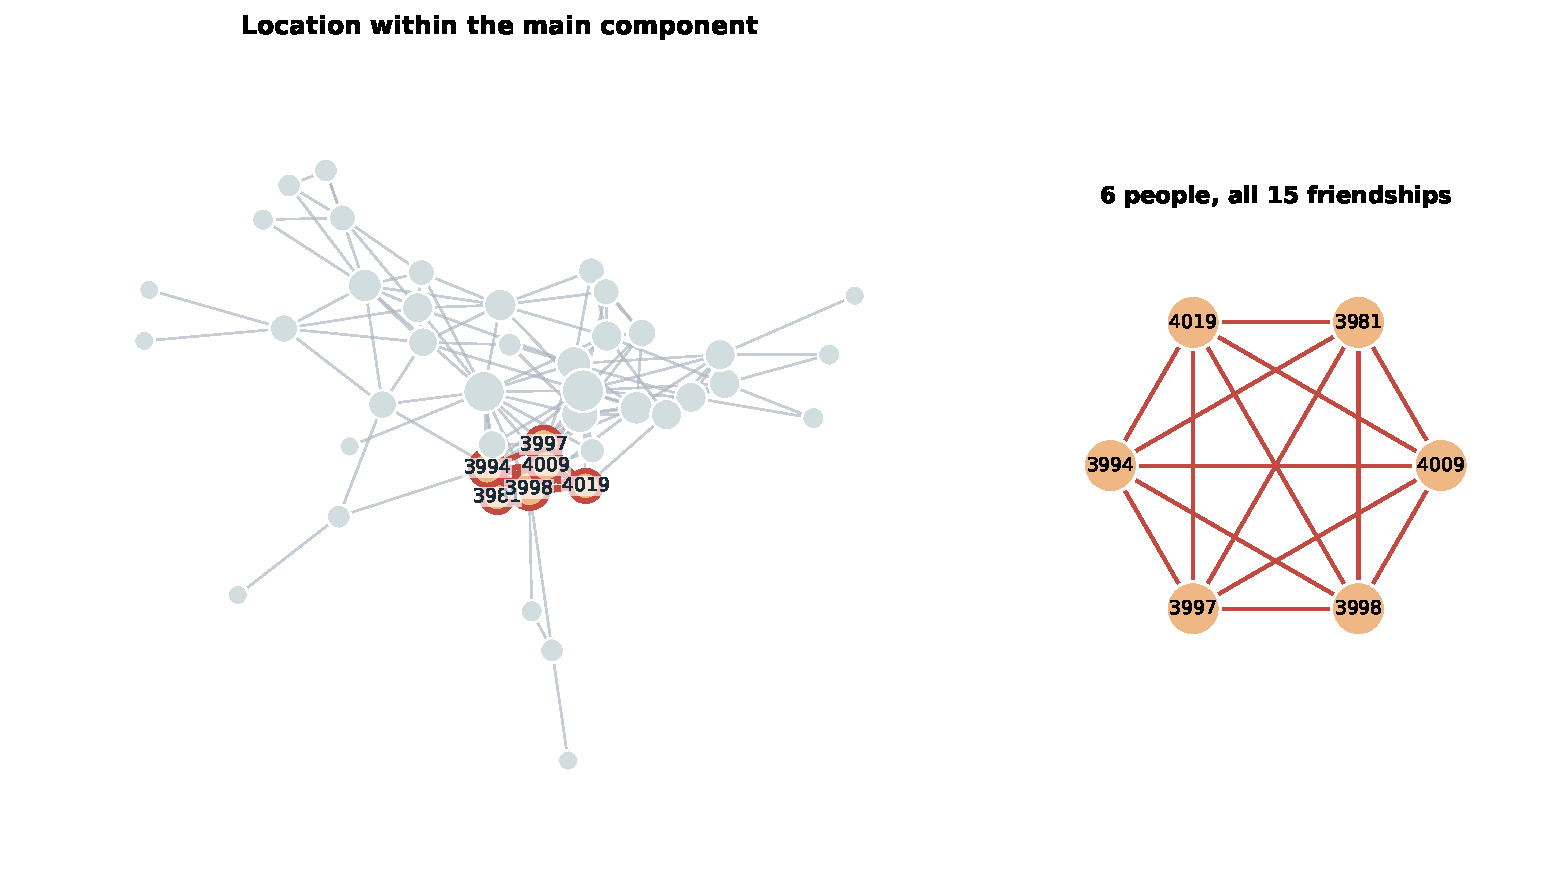
\includegraphics[width=\linewidth]{04_maximum_clique.pdf}
\caption{One maximum clique. Left: its location highlighted within the main
component. Right: a separate circular view shows all 15 friendships among its
six people. These people can also have ties outside the clique.}
\end{figure}

\clearpage
\section{Results: communities}
On the full graph, Louvain with seed 42 returns 14 groups and $Q=\FullQ{}$.
Seven of these groups are individual isolates. An isolate has degree zero, so
its community assignment does not change modularity; Louvain leaves it as a
singleton. Other groups reflect disconnected components. Thus the total count
of 14 is an algorithm output, not an estimate of 14 real social circles.
To examine finer structure, Louvain is fitted again on the main component alone.
\begin{figure}[h!]
\centering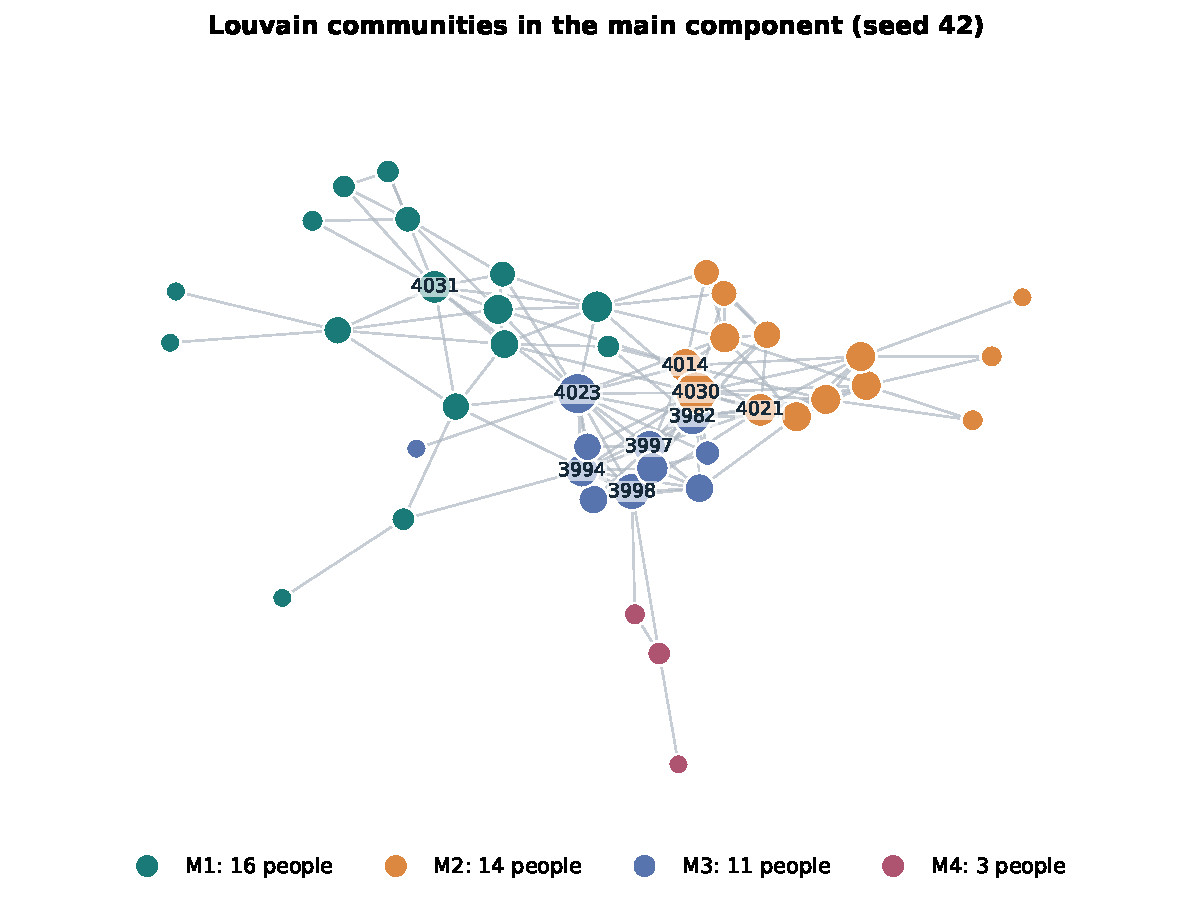
\includegraphics[width=0.94\linewidth]{02_communities.pdf}
\caption{A four-community partition of the main 44-person component, using
seed 42 and resolution 1. Sizes use the degree key in Figure~\ref{fig:overview}; only the key
people identified there are labelled. Every person's community is listed in
Appendix~\ref{app:centrality}. Colours carry no inferred family, school or workplace meaning.}
\end{figure}
\begin{table}[h!]
\centering\small\begin{tabular}{lrrrr}
\toprule
Group & People & Internal ties & External ties & Density \\
\midrule
M1 & 16 & 29 & 15 & 0.242 \\
M2 & 14 & 37 & 26 & 0.407 \\
M3 & 11 & 34 & 29 & 0.618 \\
M4 & 3 & 2 & 2 & 0.667 \\
\bottomrule
\end{tabular}

\caption{Main-component communities. External edges count ties from that group
to other groups, so a between-group edge is counted once for each endpoint group.}
\end{table}
The four groups contain 16, 14, 11 and 3 people, with $Q=\MainQ{}$. Of 138 main-
component edges, 102 are inside groups and 36 connect different groups.
M3 is a relatively dense larger group (34 of 55 possible internal ties).
M4 contains only two of three possible ties: it is a community in this partition
but is not a three-person clique. Density alone is sensitive to group size.

\clearpage
\section{Sensitivity, limitations and conclusions}
\subsection{How stable are the community results?}
Thirty additional Louvain runs on $H$, using seeds 0--29 with the same resolution,
produce four communities in \FourRunCount{} runs and five in \FiveRunCount{} runs. Their modularity values
range from \Qlow{} to \Qhigh{}. Agreement with the seed-42 partition ranges from
ARI $=\ARIlow{}$ to 1.000, showing that some membership boundaries also change.
Thus, the four-colour figure is one reproducible, plausible partition. It is not
a claim that exactly four objectively defined social groups exist. The seed-42
result was fixed for reproducibility; it was not selected as the highest-$Q$ run.

\subsection{Limits of interpretation}
\begin{itemize}
\item \textbf{Scope and selection.} This is one person's observed friend network.
The focal person is excluded and ties outside the selected group are unobserved.
The findings cannot be generalised to all Facebook users or the student's own friends.
\item \textbf{Anonymisation.} Anonymous IDs preserve source identity across
tables but cannot support labels such as family, classmates or colleagues.
No personal profile features are used to explain the communities.
\item \textbf{Disconnectedness.} The full graph has 11 components. Closeness uses
an explicit reachability correction. Eigenvector scores outside the dominant
component are effectively zero; global path statistics would be misleading.
\item \textbf{Static, binary ties.} Edges indicate recorded friendship, not its
strength, frequency or direction. There are no repeated time observations here,
so no forecasting model or claim about current friendships is justified.
\item \textbf{Algorithmic choices and validation.} Louvain depends on random
order and resolution. Modularity is a descriptive objective, not a significance
test. The source includes ego-defined circle memberships, but this report does
not compare the detected communities with that reference. Their agreement has
therefore not been assessed. Anonymous circle names do not identify social meaning.
\end{itemize}

\subsection{Conclusions}
Within the selected graph, person 4030 has the most direct ties and person 4023
ranks highest on betweenness. Six maximum six-person cliques overlap across
15 distinct people. Louvain yields four or five groups inside the main connected
component across the tested seeds. The network therefore combines several
disconnected components, tightly connected local groups and people with distinct
structural roles; no one centrality ranking captures all of those properties.

\clearpage
\section{Reproducing the analysis}
The accompanying project contains the full data preparation, calculations,
visualisations and exported tables. It was run with Python \PythonVersion{},
NetworkX \NetworkXVersion{}, Matplotlib \MatplotlibVersion{}, NumPy \NumpyVersion{}
and SciPy \ScipyVersion{}. The exact dependency versions are in
\texttt{requirements.txt}. From the extracted project directory:
\begin{lstlisting}[language=bash,numbers=none]
python -m pip install -r requirements.txt
python network_analysis.py
\end{lstlisting}
The bundled archive permits this second command to run offline. The script
recreates prepared CSVs in \texttt{data/}, numerical outputs in \texttt{results/}
and vector PDF plus PNG figures in \texttt{figures/}. Tables retain more decimal
places than the rounded report. \texttt{run\_analysis.ipynb} provides a notebook
entry point. Rebuilding this report additionally requires a LaTeX installation;
instructions are in \texttt{README.txt}.

Validation includes the handshaking identity $\sum_i k_i=2m$, triangle counts
from two algorithms, pairwise completeness of enumerated maximal cliques,
and PageRank probabilities summing to one. The optional
\texttt{verify\_results.py} independently checks the saved outputs using
direct shortest-path enumeration, matrix calculations and recursive clique
enumeration. It saves \texttt{results/verification.json}.
Complete analysis and plotting code
appears in Appendix~\ref{app:code}.

\begin{thebibliography}{9}\small
\bibitem{snap} Stanford Network Analysis Project. \emph{Social circles: Facebook}.
Dataset and file-format documentation. Accessed 6 November 2026.
\url{https://snap.stanford.edu/data/ego-Facebook.html} and
\url{https://snap.stanford.edu/data/readme-Ego.txt}.
\bibitem{mcauley} McAuley, J. and Leskovec, J. (2012).
Learning to Discover Social Circles in Ego Networks.
\emph{Advances in Neural Information Processing Systems}, 25.
\bibitem{blondel} Blondel, V. D., Guillaume, J.-L., Lambiotte, R. and
Lefebvre, E. (2008). Fast unfolding of communities in large networks.
\emph{Journal of Statistical Mechanics}, P10008.
\url{https://doi.org/10.1088/1742-5468/2008/10/P10008}.
\bibitem{nxcentrality} NetworkX Developers. Centrality documentation, including
normalisation and disconnected-graph conventions.
\url{https://networkx.org/documentation/stable/reference/algorithms/centrality.html}.
\bibitem{nxpagerank} NetworkX Developers. \texttt{pagerank} documentation.
\url{https://networkx.org/documentation/stable/reference/algorithms/generated/networkx.algorithms.link_analysis.pagerank_alg.pagerank.html}.
\bibitem{nxcliques} NetworkX Developers. \texttt{find\_cliques} documentation.
\url{https://networkx.org/documentation/stable/reference/algorithms/generated/networkx.algorithms.clique.find_cliques.html}.
\bibitem{nxlouvain} NetworkX Developers. \texttt{louvain\_communities} documentation.
\url{https://networkx.org/documentation/stable/reference/algorithms/generated/networkx.algorithms.community.louvain.louvain_communities.html}.
\bibitem{lecture} Kavaliauskas, M. (2025). \emph{Graph and network analysis}.
KTU lecture slides, 28 October 2025. Supplied with the assignment.
\end{thebibliography}

\clearpage
\appendix
\section{Centrality values for all 59 people}\label{app:centrality}
Values are rounded to four decimals and use the full graph. Comp. denotes
connected component. F denotes a community fitted on all 59 people; M denotes a
community fitted separately on the 44-node main component, both using seed 42.
A dash means the person is outside that main component. Components and community
labels are numbered by decreasing size, with minimum ID breaking ties.
The CSV files preserve full precision. A printed zero for eigenvector
centrality can represent a very small numerical value outside the dominant component.
\begingroup\fontsize{8.5}{10}\selectfont
\renewcommand{\arraystretch}{0.96}
\setlength{\tabcolsep}{4.5pt}
\begin{longtable}{rrrrrrrrrr}
\toprule
ID & $k$ & $D$ & $C$ & $B$ & $E$ & $P$ & Comp. & F & M \\
\midrule
\endfirsthead
\toprule
ID & $k$ & $D$ & $C$ & $B$ & $E$ & $P$ & Comp. & F & M \\
\midrule
\endhead
\bottomrule
\endfoot
594 & 3 & 0.0517 & 0.2397 & 0.0003 & 0.0142 & 0.0123 & 1 & 1 & 1 \\
3981 & 7 & 0.1207 & 0.3065 & 0.0009 & 0.1771 & 0.0186 & 1 & 2 & 3 \\
3982 & 13 & 0.2241 & 0.3707 & 0.0283 & 0.2949 & 0.0328 & 1 & 2 & 3 \\
3983 & 1 & 0.0172 & 0.2214 & 0.0000 & 0.0148 & 0.0054 & 1 & 3 & 2 \\
3984 & 0 & 0.0000 & 0.0000 & 0.0000 & 0.0000 & 0.0028 & 5 & 8 & -- \\
3985 & 5 & 0.0862 & 0.2872 & 0.0014 & 0.0760 & 0.0145 & 1 & 4 & 2 \\
3986 & 8 & 0.1379 & 0.3125 & 0.0161 & 0.1672 & 0.0221 & 1 & 3 & 2 \\
3987 & 1 & 0.0172 & 0.0172 & 0.0000 & 0.0000 & 0.0189 & 3 & 6 & -- \\
3988 & 6 & 0.1034 & 0.2925 & 0.0030 & 0.1243 & 0.0165 & 1 & 4 & 2 \\
3989 & 5 & 0.0862 & 0.2510 & 0.0044 & 0.0235 & 0.0188 & 1 & 1 & 1 \\
3990 & 3 & 0.0517 & 0.0517 & 0.0000 & 0.0000 & 0.0189 & 2 & 5 & -- \\
3991 & 2 & 0.0345 & 0.2379 & 0.0003 & 0.0127 & 0.0088 & 1 & 1 & 1 \\
3992 & 2 & 0.0345 & 0.2261 & 0.0000 & 0.0289 & 0.0079 & 1 & 3 & 2 \\
3993 & 5 & 0.0862 & 0.2952 & 0.0014 & 0.0881 & 0.0144 & 1 & 4 & 2 \\
3994 & 10 & 0.1724 & 0.3542 & 0.0316 & 0.2427 & 0.0267 & 1 & 2 & 3 \\
3995 & 8 & 0.1379 & 0.3356 & 0.0153 & 0.1360 & 0.0217 & 1 & 4 & 2 \\
3996 & 3 & 0.0517 & 0.2725 & 0.0259 & 0.0356 & 0.0136 & 1 & 1 & 1 \\
3997 & 10 & 0.1724 & 0.3503 & 0.0047 & 0.2609 & 0.0252 & 1 & 2 & 3 \\
3998 & 13 & 0.2241 & 0.3795 & 0.0886 & 0.2634 & 0.0363 & 1 & 2 & 3 \\
3999 & 3 & 0.0517 & 0.2592 & 0.0254 & 0.0315 & 0.0154 & 1 & 2 & 4 \\
4000 & 8 & 0.1379 & 0.3036 & 0.0209 & 0.1330 & 0.0232 & 1 & 3 & 2 \\
4001 & 1 & 0.0172 & 0.0172 & 0.0000 & 0.0000 & 0.0189 & 4 & 7 & -- \\
4002 & 6 & 0.1034 & 0.3356 & 0.0427 & 0.0903 & 0.0202 & 1 & 1 & 1 \\
4003 & 4 & 0.0690 & 0.3125 & 0.0000 & 0.1275 & 0.0115 & 1 & 2 & 3 \\
4004 & 9 & 0.1552 & 0.3582 & 0.0292 & 0.1427 & 0.0252 & 1 & 4 & 1 \\
4005 & 2 & 0.0345 & 0.2571 & 0.0000 & 0.0312 & 0.0096 & 1 & 2 & 4 \\
4006 & 1 & 0.0172 & 0.2111 & 0.0000 & 0.0045 & 0.0063 & 1 & 1 & 1 \\
4007 & 3 & 0.0517 & 0.0517 & 0.0000 & 0.0000 & 0.0189 & 2 & 5 & -- \\
4008 & 0 & 0.0000 & 0.0000 & 0.0000 & 0.0000 & 0.0028 & 6 & 9 & -- \\
4009 & 9 & 0.1552 & 0.3465 & 0.0041 & 0.2351 & 0.0231 & 1 & 2 & 3 \\
4010 & 0 & 0.0000 & 0.0000 & 0.0000 & 0.0000 & 0.0028 & 7 & 10 & -- \\
4011 & 3 & 0.0517 & 0.2397 & 0.0003 & 0.0142 & 0.0123 & 1 & 1 & 1 \\
4012 & 1 & 0.0172 & 0.0172 & 0.0000 & 0.0000 & 0.0189 & 3 & 6 & -- \\
4013 & 5 & 0.0862 & 0.3065 & 0.0061 & 0.0732 & 0.0160 & 1 & 1 & 1 \\
4014 & 11 & 0.1897 & 0.3795 & 0.0522 & 0.2277 & 0.0290 & 1 & 3 & 2 \\
4015 & 0 & 0.0000 & 0.0000 & 0.0000 & 0.0000 & 0.0028 & 8 & 11 & -- \\
4016 & 3 & 0.0517 & 0.0517 & 0.0000 & 0.0000 & 0.0189 & 2 & 5 & -- \\
4017 & 8 & 0.1379 & 0.3125 & 0.0392 & 0.1401 & 0.0244 & 1 & 3 & 2 \\
4018 & 6 & 0.1034 & 0.3321 & 0.0010 & 0.1713 & 0.0162 & 1 & 2 & 3 \\
4019 & 7 & 0.1207 & 0.3095 & 0.0038 & 0.1805 & 0.0184 & 1 & 2 & 3 \\
4020 & 7 & 0.1207 & 0.3582 & 0.0338 & 0.0952 & 0.0218 & 1 & 1 & 1 \\
4021 & 10 & 0.1724 & 0.3356 & 0.0178 & 0.2262 & 0.0258 & 1 & 3 & 2 \\
4022 & 0 & 0.0000 & 0.0000 & 0.0000 & 0.0000 & 0.0028 & 9 & 12 & -- \\
4023 & 17 & 0.2931 & 0.4195 & 0.1228 & 0.3211 & 0.0453 & 1 & 2 & 3 \\
4024 & 0 & 0.0000 & 0.0000 & 0.0000 & 0.0000 & 0.0028 & 10 & 13 & -- \\
4025 & 3 & 0.0517 & 0.0517 & 0.0000 & 0.0000 & 0.0189 & 2 & 5 & -- \\
4026 & 8 & 0.1379 & 0.3095 & 0.0047 & 0.1726 & 0.0212 & 1 & 3 & 2 \\
4027 & 6 & 0.1034 & 0.2925 & 0.0508 & 0.0422 & 0.0244 & 1 & 1 & 1 \\
4028 & 1 & 0.0172 & 0.2005 & 0.0000 & 0.0038 & 0.0067 & 1 & 1 & 1 \\
4029 & 1 & 0.0172 & 0.0172 & 0.0000 & 0.0000 & 0.0189 & 4 & 7 & -- \\
4030 & 18 & 0.3103 & 0.4035 & 0.1042 & 0.3544 & 0.0447 & 1 & 3 & 2 \\
4031 & 10 & 0.1724 & 0.3391 & 0.0776 & 0.0967 & 0.0324 & 1 & 1 & 1 \\
4032 & 1 & 0.0172 & 0.2111 & 0.0000 & 0.0045 & 0.0063 & 1 & 1 & 1 \\
4033 & 2 & 0.0345 & 0.2261 & 0.0000 & 0.0317 & 0.0076 & 1 & 3 & 2 \\
4034 & 1 & 0.0172 & 0.2702 & 0.0000 & 0.0340 & 0.0051 & 1 & 2 & 3 \\
4035 & 0 & 0.0000 & 0.0000 & 0.0000 & 0.0000 & 0.0028 & 11 & 14 & -- \\
4036 & 1 & 0.0172 & 0.1932 & 0.0000 & 0.0033 & 0.0072 & 1 & 2 & 4 \\
4037 & 3 & 0.0517 & 0.3007 & 0.0008 & 0.0653 & 0.0099 & 1 & 1 & 1 \\
4038 & 8 & 0.1379 & 0.3465 & 0.0368 & 0.1081 & 0.0245 & 1 & 1 & 1 \\
\end{longtable}

\endgroup

\clearpage
\section{Complete Python analysis and plotting code}\label{app:code}
The following is the entire \texttt{network\_analysis.py} file used for the report.
It prepares the data, computes both graph scopes, enumerates cliques, runs
community sensitivity analysis, writes numerical outputs and creates every plot.
Report typesetting files are included separately in the project bundle.
\lstinputlisting{../network_analysis.py}
\end{document}
